% Chapter 3
\chapter[ỨNG DỤNG HADOOP MAPREDUCE VỚI ITEM-BASED COLLABORATIVE FILTERING TRONG RECOMMENDATION SYSTEM]
 {\LARGE ỨNG DỤNG HADOOP MAPREDUCE VỚI ITEM-BASED COLLABORATIVE FILTERING TRONG RECOMMENDATION SYSTEM}

% Section 1 Chapter 3
\section{Ý tưởng MapReduce Item-based Collaborative Filtering}
\textbf{Nhiệm vụ}: MapReduce chia quá trình tính toán thành các bước nhỏ hơn \\
\hspace*{2cm}(Map và Reduce), cho phép xử lý song song dữ liệu lớn. \\
\vspace{0.5cm}
\textbf{Ý tưởng}: Phân tán việc tính toán ma trận đồng xuất hiện và ma trận đánh \\
\hspace*{1.7cm}giá qua nhiều máy tính \\
\hspace*{1.7cm}$\rightarrow$ giảm thời gian xử lý và tăng hiệu suất \\
\hspace*{1.7cm}$\rightarrow$ giải quyết các thách thức về kích thước dữ liệu và độ phức tạp của tính toán trong hệ thống gợi ý

% Section 2 Chapter 3
\section{Lưu đồ của thuật toán MapReduce Item-based Collaborative Filtering}
\vspace*{-1cm}
\begin{figure}[ht]
    \centering
    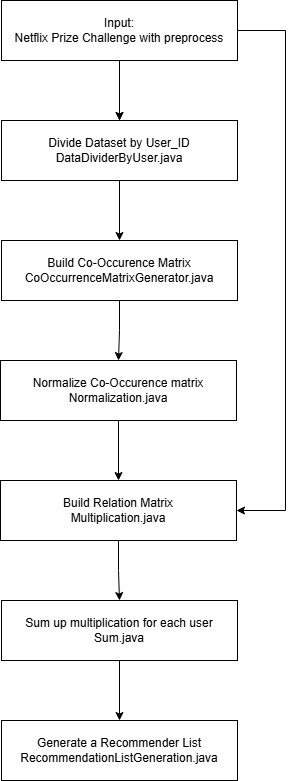
\includegraphics[width=4cm]{images/RecommenderSystem.jpg}
    \caption{Lưu đồ thuật toán Mapreduce Item-based Collaborative Filtering}
\end{figure}
% Section 3 Chapter 3
\section{Triển khai thuật toán MapReduce Item-based Collaborative Filtering}
\subsection*{Giải pháp Mapreduce cho Item-based Collaborative Filtering}
\begin{itemize}
    \item \textbf{Dữ liệu đầu vào}: Là danh sách các hàng lưu dưới dạng file .txt.
          Mỗi hàng chứa thông tin về người dùng, sản phẩm và đánh giá của người dùng đó
          cho sản phẩm đó, cách nhau bởi dấu phẩy, được chuyển sang kiểu key-value làm
          đầu vào cho thuật toán
    \item \textbf{Triển khai}:
          \begin{enumerate}
              \item Biểu diễn dữ liệu. Dữ liệu lưu trữ dưới dạng list các hàng. Mỗi hàng
                    chứa thông tin về người dùng, sản phẩm và đánh giá của người dùng đó cho
                    sản phẩm đó, cách nhau bởi dấu phẩy.
              \item Lưu trữ phân tán dữ liệu. Dữ liệu được chia thành các phần nhỏ và lưu trữ
                    trên nhiều máy tính khác nhau.
              \item Trên mỗi máy tính, trong mỗi vòng lặp, thực hiện đọc vào từng dòng,
                    gửi lại kết quả cho reducer để tính độ lợi thông tin của từng thuộc tính trong từng phần dữ liệu.
              \item Thực hiện gọi đệ quy xác định nút gốc và nút lá tương ứng.
                    Cập nhật lại nút, cho đến khi đạt hội tụ sau mỗi vòng lặp.\\
                    \vspace{0.2cm}
                    \hspace*{-1cm} $\implies$ \textit{Dữ liệu cần phân lớp}: Là danh sách các hàng lưu trên file .txt. được chuyển sang kiểu key/value làm đầu ra cho thuật toán.
          \end{enumerate}
    \item \textbf{Mô hình cơ bản của MapReduce}:
          \begin{itemize}
              \item Map (KeyIn, ValIn) $\rightarrow$ List(KeyInt, ValInt)
              \item Reduce (KeyInt, List(ValInt)) $\rightarrow$ List(KeyOut, ValOut)
          \end{itemize}
    \item \textbf{Áp dụng cho thuật toán Item-based Collaborative Filtering}:
          \begin{itemize}
              \item Xây dựng lớp DataDividedByUser
              \item Xây dựng lớp CoOccurrenceMatrixGenerator
              \item Xây dựng lớp Normalize
              \item Xây dựng lớp Multiplication
              \item Xây dựng lớp Sum
              \item Xây dựng lớp RecommendationListGenerator
              \item Xây dựng lớp RecommendationListName
              \item Xây dựng lớp RecommendationName
          \end{itemize}
\end{itemize}

\subsection*{Bước 1: Xây dựng lớp DataDividerByUser}
\begin{itemize}
    \item \textbf{Xử lý}: Nhóm movie và rating tương ứng theo user \\
    \item \textbf{Mapper}
          \begin{itemize}
              \item \textbf{Input}: user, movie, rating \\
              \item \textbf{Output}: key là user, value là movie:rating \\
          \end{itemize}
    \item \textbf{Reducer}
          \begin{itemize}
              \item \textbf{Input}: key là user, value là movie:rating \\
              \item \textbf{Output}: user \quad movie1:rating1, movie2:rating2, ... \\
          \end{itemize}
\end{itemize}
\subsection*{Bước 2: Xây dựng lớp CoOccurrenceMatrixGenerator}
\begin{itemize}
    \item \textbf{Xử lý}: Đếm số lần mỗi cặp movie được đánh giá bởi cùng 1 người \\
    \item \textbf{Mapper}
          \begin{itemize}
              \item \textbf{Input}: user \quad movie1:rating1, movie2:rating2, ... \\
              \item \textbf{Output}: key là movie1:movie2, value là 1 \\
          \end{itemize}
    \item \textbf{Reducer}
          \begin{itemize}
              \item \textbf{Input}: key là movie1:movie2, value là 1 \\
              \item \textbf{Output}: movie1:movie2 \quad count (trong đó
                    count là số lần cặp movie đó được đánh giá bởi cùng 1 người) \\
          \end{itemize}
\end{itemize}
\subsection*{Bước 3: Xây dựng lớp Normalize}
\begin{itemize}
    \item \textbf{Xử lý}: Chuẩn hóa từng đơn vị của ma trận đồng xuất hiện
          bằng cách chia giá trị đó cho tổng giá trị của cột tương ứng trong ma trận
    \item \textbf{Mapper}
          \begin{itemize}
              \item \textbf{Input}: movie1:movie2 \quad count \\
              \item \textbf{Output}: key là movie1, value là movie2:count \\
          \end{itemize}
    \item \textbf{Reducer}
          \begin{itemize}
              \item \textbf{Input}: key là movie1, value là movie2:count \\
              \item \textbf{Output}: movie1 \quad movie2=relation (với relation
                    là giá trị sau khi xử lý) \\
          \end{itemize}
\end{itemize}
\subsection*{Bước 4: Xây dựng lớp Multiplication}
\begin{itemize}
    \item \textbf{Xử lý}: Nhân relation với rating tương ứng với mỗi key là movie
    \item \textbf{CooccurrenceMapper}
          \begin{itemize}
              \item \textbf{Input}: movie1 \quad movie2=relation \\
              \item \textbf{Output}: key là movie1, value là movie2=relation \\
          \end{itemize}
    \item \textbf{RatingMapper}
          \begin{itemize}
              \item \textbf{Input}: user, movie, rating \\
              \item \textbf{Output}: key là movie, value là user:rating \\
          \end{itemize}
    \item \textbf{Reducer}
          \begin{itemize}
              \item \textbf{Input}: key là movie, value là movie1=relation, movie2=relation, ..., userA:rating, userB:rating, ... \\
              \item \textbf{Output}: user:movie \quad result (với $result = relation \times rating$) \\
          \end{itemize}
\end{itemize}
\subsection*{Bước 5: Xây dựng lớp Sum}
\begin{itemize}
    \item \textbf{Xử lý}: Tính tổng các result theo key là user:movie
    \item \textbf{Mapper}
          \begin{itemize}
              \item \textbf{Input}: user:movie \quad result \\
              \item \textbf{Output}: key là user:movie, value là result \\
          \end{itemize}
    \item \textbf{Reducer}
          \begin{itemize}
              \item \textbf{Input}: key là user:movie, value là result \\
              \item \textbf{Output}: user:movie \quad sum (với sum là tổng các result) \\
          \end{itemize}
\end{itemize}
\subsection*{Bước 6: Xây dựng lớp RecommendationListGenerator}
\begin{itemize}
    \item \textbf{Xử lý}: Lấy ra k movie có giá trị sum lớn nhất với mỗi user được sắp xếp giảm dần (ở đây chúng em lấy k=5)
    \item \textbf{Mapper}
          \begin{itemize}
              \item \textbf{Input}: user:movie \quad sum \\
              \item \textbf{Output}: key là user, value là movie:sum \\
          \end{itemize}
    \item \textbf{Reducer}
          \begin{itemize}
              \item \textbf{Input}: key là user, value là movie:sum \\
              \item \textbf{Output}: user \quad movie:sum
          \end{itemize}
\end{itemize}
\subsection*{Bước 7: Xây dựng lớp RecommendationListName}
\begin{itemize}
    \item \textbf{Xử lý}: Thay thế movie trong RecommendationListGenerator bằng tên movie tương ứng trong movie\_titles.txt
    \item \textbf{RecommendationListMapper}
          \begin{itemize}
              \item \textbf{Input}: user \quad movie:sum \\
              \item \textbf{Output}: key là movie, value là user=movie=sum \\
          \end{itemize}
    \item \textbf{TitlesMapper}
          \begin{itemize}
              \item \textbf{Input}: movie,name \\
              \item \textbf{Output}: key là movie, value là movie:name \\
          \end{itemize}
    \item \textbf{Reducer}
          \begin{itemize}
              \item \textbf{Input}: key là movie, value là userA=movie1=sum, userB=movie2=sum, ..., movie1:name1, movie2:name2, ... \\
              \item \textbf{Output}: user \quad name:sum\\
          \end{itemize}
\end{itemize}
\subsection*{Bước 8: Xây dựng lớp RecommendationName}
\begin{itemize}
    \item \textbf{Xử lý}: Sắp xếp lại RecommendationListName theo userID tăng dần và sum giảm dần
    \item \textbf{Mapper}
          \begin{itemize}
              \item \textbf{Input}: user \quad name:sum \\
              \item \textbf{Output}: key là user, value là name:sum \\
          \end{itemize}
    \item \textbf{Reducer}
          \begin{itemize}
              \item \textbf{Input}: key là user, value là name:sum \\
              \item \textbf{Output}: user \quad name \\
          \end{itemize}
\end{itemize}

% Section 4 Chapter 3
\pagebreak
\section{Demo thuật toán MapReduce Item-based Collaborative Filtering}
\subsection*{Demo cài đặt hadoop thành công}
\begin{figure}[h]
    \centering
    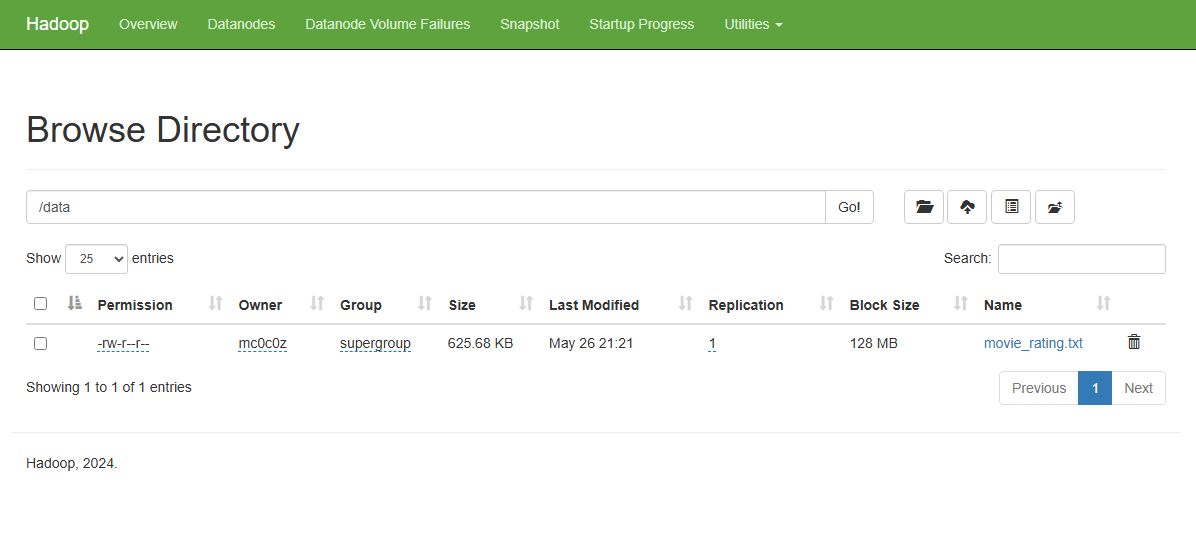
\includegraphics[width=12cm]{images/Demo1.png}
    \caption{Demo cài đặt Hadoop thành công}
\end{figure}
\subsection*{Demo Chương trình}
\begin{enumerate}
    \item Cấu trúc thư mục của Project
          \begin{figure}[h]
              \centering
              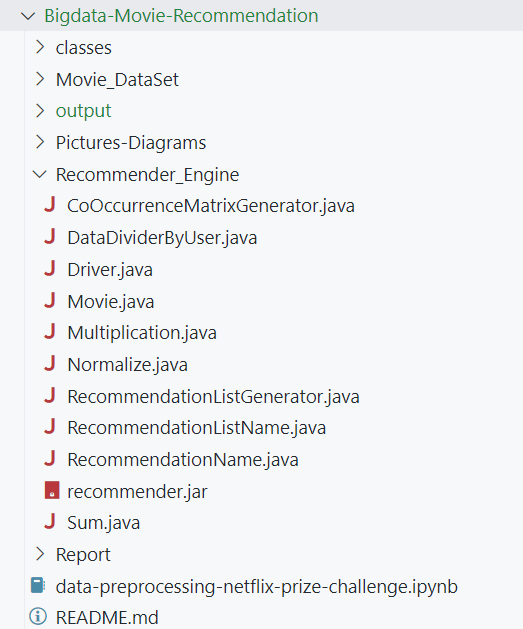
\includegraphics[width=6cm]{images/Demo2.png}
              \caption{Cấu trúc thư mục của Project}
          \end{figure}
          \pagebreak
    \item Kết quả chương trình
          \begin{figure}[ht]
              \centering
              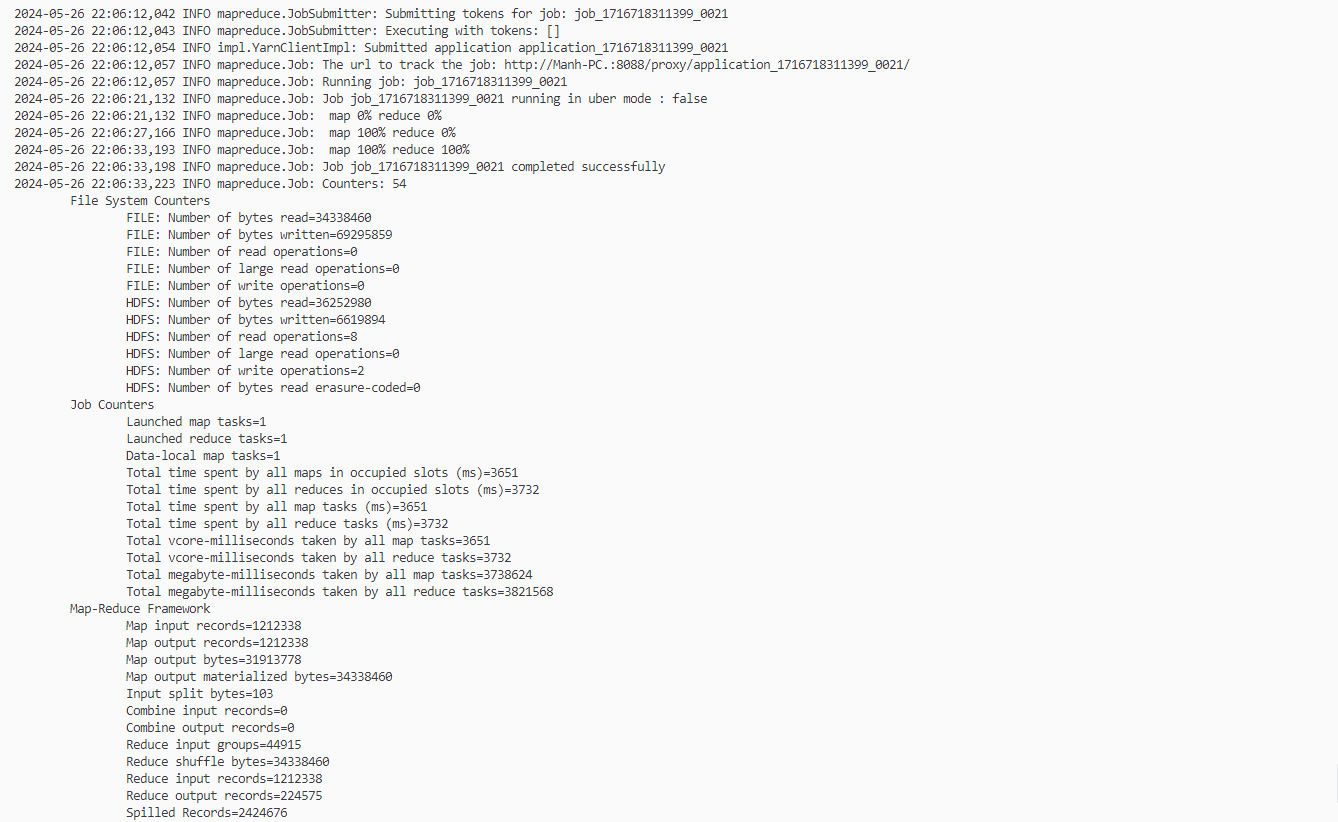
\includegraphics[width=15cm]{images/Demo3.png}
              \caption{Kết quả chương trình}
          \end{figure}
    \item File kết quả đầu ra
          \begin{figure}[ht]
              \centering
              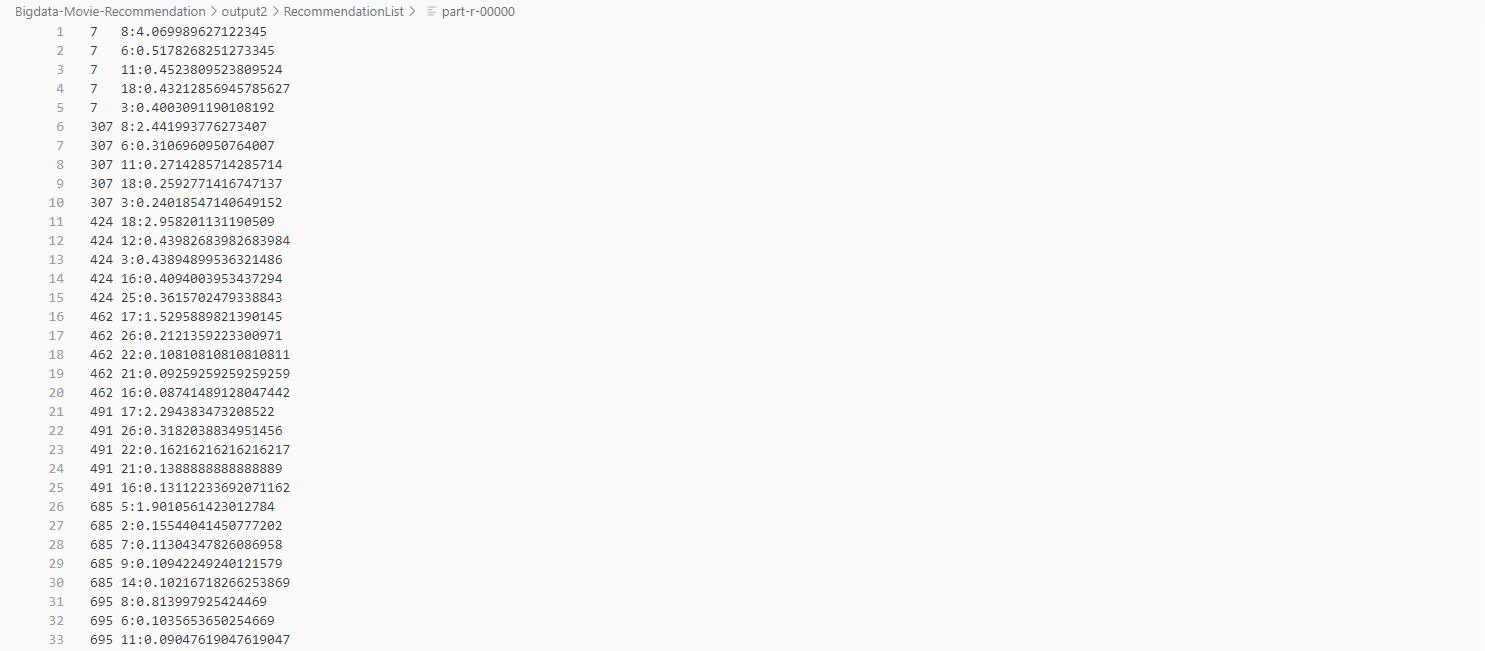
\includegraphics[width=15cm]{images/Demo4.png}
              \caption{File kết quả đầu ra}
          \end{figure}
    \item Đánh giá
          \begin{itemize}
              \item Chương trình đã chạy thành công thuật toán MapReduce Item-based Collaborative Filtering.
              \item Kết quả chạy khớp với kết quả đã thực hiện thủ công trước đó \\ $\rightarrow$ có triển vọng mở rộng với tập dữ liệu lớn hơn
          \end{itemize}
\end{enumerate}
